\section{Trực quan hóa phân bố dữ liệu thực nghiệm}
\label{sec:truc_quan_hoa_du_lieu}

Quá trình trực quan hóa dữ liệu là công đoạn cơ bản trong quy trình phân tích của các hệ thống đo lường tự động. Thay vì làm việc với các bảng dữ liệu quy mô nhỏ, các mảng dữ liệu được nạp từ tệp \texttt{.csv} (như thời gian, độ dịch chuyển và vận tốc) cần được ánh xạ vào không gian tọa độ. Thao tác này hỗ trợ việc đánh giá khách quan đặc tính quỹ đạo và mức độ phân tán của dữ liệu trước khi tiến hành tính toán lan truyền sai số và hồi quy mô hình. Đối với bài toán minh họa rơi tự do, bước này giúp xác nhận sơ bộ tính chất parabol của tọa độ và tính tuyến tính của đại lượng vận tốc.

\begin{physcore}{Khái niệm điểm dữ liệu và vùng bất định đo lường}{data_point_uncertainty}
Trong khuôn khổ của vật lý thực nghiệm và đo lường học, một điểm dữ liệu (data point) không được định nghĩa là một tọa độ vô hướng đơn thuần trên mặt phẳng toán học. Bản chất của mỗi điểm dữ liệu là một vùng bất định (uncertainty region), được giới hạn bởi các giá trị sai số hệ thống (systematic errors) từ thiết bị cảm biến. Đối với các hệ thống lấy mẫu tự động, giới hạn độ phân giải không gian và thời gian tạo thành các ranh giới vi mô bao quanh mỗi kết quả ghi nhận.
\end{physcore}

Để triển khai nguyên lý này trên môi trường lập trình, thư viện \texttt{matplotlib} được sử dụng nhằm mục đích cấu trúc hóa các đại lượng động học thành đối tượng đồ họa. Việc cấu hình các tham số hiển thị toàn cục (như phông chữ chuẩn LaTeX và độ phân giải) là yêu cầu thiết yếu nhằm đảm bảo đồ thị đầu ra đáp ứng tiêu chuẩn xuất bản khoa học.

\begin{pycode}{High-resolution visualization of sensor data}
import matplotlib.pyplot as plt

# Global configuration for high-resolution scientific plotting
plt.rcParams.update({
    "text.usetex": True,            
    "font.family": "serif",        
    "font.serif": ["Computer Modern Roman"],
    "figure.dpi": 150,              
    "axes.labelsize": 12,       
    "font.size": 12,              
    "legend.fontsize": 10,     
    "xtick.labelsize": 10,         
    "ytick.labelsize": 10,        
    "axes.titlesize": 14,          
    "lines.linewidth": 1.5,        
    "grid.alpha": 0.5,              
    "grid.linestyle": "--"          
})

# Setup graphical structures
fig, (ax1, ax2) = plt.subplots(1, 2, figsize=(12, 5))

# Visualization 1: Displacement vs Time
ax1.scatter(time_data, displacement_data, color='black', edgecolor='blue', 
            label=r'$\mathrm{Experimental \ Coordinates}$')
ax1.set_xlabel(r'$\mathrm{Time} \ t \ (\mathrm{s})$')
ax1.set_ylabel(r'$\mathrm{Displacement} \ s \ (\mathrm{m})$')
ax1.set_title(r'$\mathrm{Free \ Fall \ Kinematics: \ Position}$')
ax1.legend()
ax1.grid(True, linestyle=':', alpha=0.7)

# Visualization 2: Velocity vs Time
ax2.scatter(time_midpoints, velocity_data, color='black', edgecolor='green', 
            label=r'$\mathrm{Derived \ Velocity}$')
ax2.set_xlabel(r'$\mathrm{Time} \ t \ (\mathrm{s})$')
ax2.set_ylabel(r'$\mathrm{Velocity} \ v \ (\mathrm{m/s})$')
ax2.set_title(r'$\mathrm{Free \ Fall \ Kinematics: \ Velocity}$')
ax2.legend()
ax2.grid(True, linestyle=':', alpha=0.7)

plt.tight_layout()
plt.show()
\end{pycode}

\begin{figure}[htbp]
    \centering
    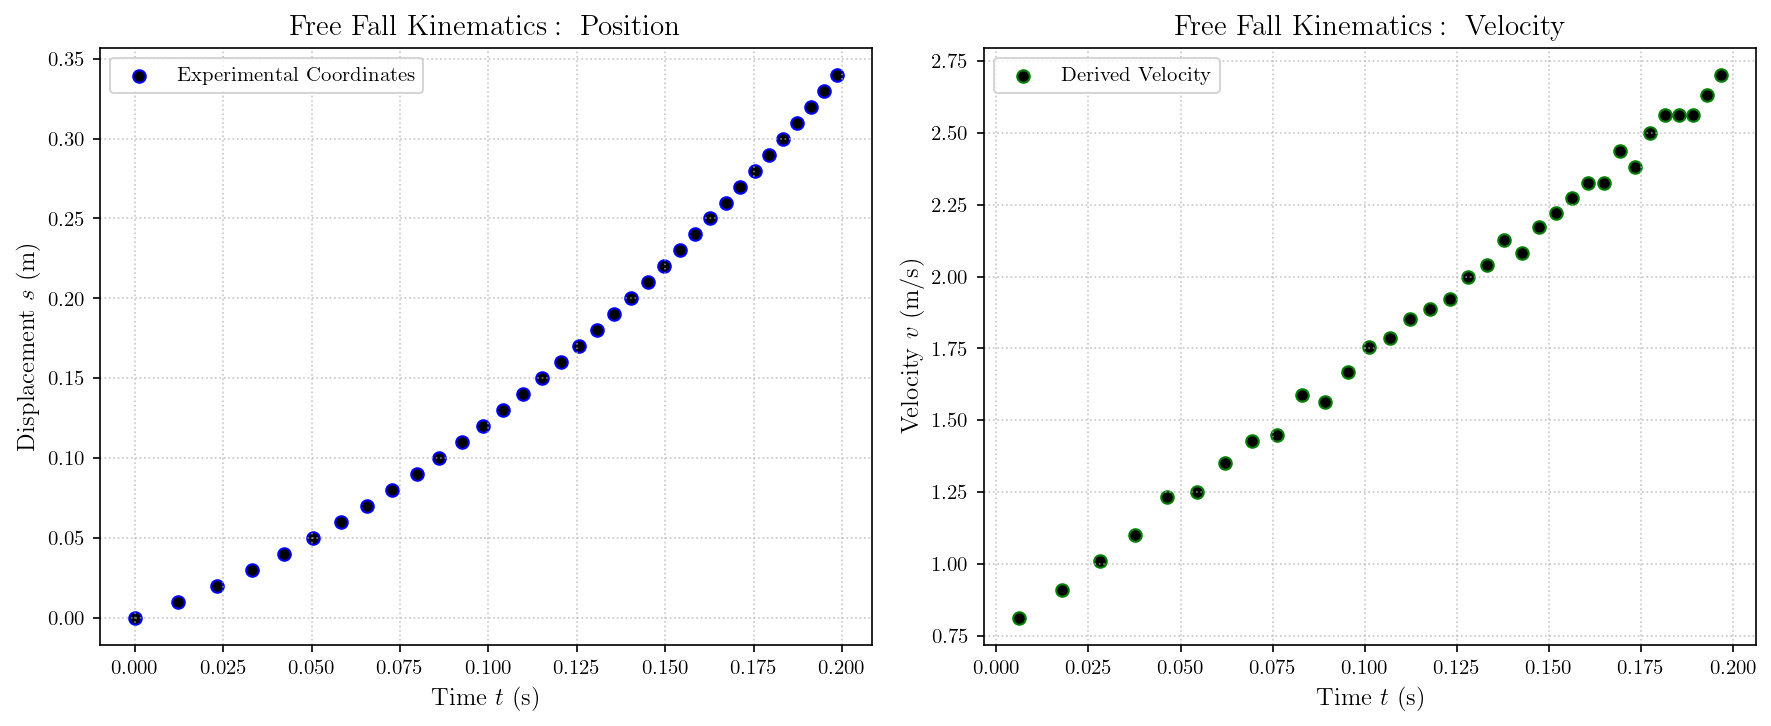
\includegraphics[width=\textwidth]{figures/fig_raw_kinematics.png}
    \caption{Trực quan hóa phân bố dữ liệu thực nghiệm ban đầu của độ dịch chuyển và vận tốc dẫn xuất.}
    \label{fig:raw_kinematics_plot}
\end{figure}

Đoạn mã trên minh họa kỹ thuật thiết lập biểu đồ song song (subplots) cho cả hai nhóm đại lượng: vị trí đo lường trực tiếp và vận tốc dẫn xuất. Việc định dạng nhãn trục tọa độ được thực hiện thông qua cấu trúc chuỗi thô (raw strings) mang tiền tố \texttt{r} kết hợp cú pháp toán học LaTeX. Ở giai đoạn này, không gian phân bố vĩ mô của tập dữ liệu đã được xác lập, tạo nền tảng trực quan để lồng ghép các đường cong mô hình lý thuyết và thanh sai số cục bộ trong các bước phân tích chuyên sâu.

% \begin{pitfall}{Che khuất vùng bất định trong dữ liệu mật độ cao}{error_bar_representation}
\begin{pitfall}{Hiện tượng che lấp thanh sai số trong không gian dữ liệu mật độ cao}{error_bar_representation}
Bước thiết lập đồ thị đối với các mảng dữ liệu lấy mẫu tự động thường tiềm ẩn rủi ro về mặt biểu diễn thị giác. Do số lượng điểm quan trắc lớn và độ bất định thiết bị ở mức vi mô, việc rải thanh sai số trực tiếp lên toàn bộ đồ thị vĩ mô dễ gây ra hiện tượng nhiễu hình ảnh, hoặc các thanh sai số bị che lấp bởi chính các điểm đánh dấu (marker). Phương pháp biểu diễn này làm giảm khả năng nhận diện các giới hạn sai số đo lường. Để khắc phục, một giải pháp đồ họa tối ưu là duy trì việc vẽ điểm ở góc nhìn toàn cảnh, đồng thời sử dụng kỹ thuật trục phụ nội tuyến (inset axes) để phóng to một vùng dữ liệu cục bộ (phương pháp này sẽ được tích hợp chi tiết tại chương hồi quy mô hình), giúp minh chứng rõ ràng sự hiện diện của giới hạn phân giải thiết bị.
\end{pitfall}